% 2x2 framework diagram crossing Novelty x Specificity to define A1-A4.
%
%   Rows:    Novelty     (No: continued availability | Yes: new introduction)
%   Columns: Specificity (No: ABF sales              | Yes: counterpart sales)
%
%   A1 = (no  novelty, no  specificity)   A2 = (no  novelty, yes specificity)
%   A3 = (yes novelty, no  specificity)   A4 = (yes novelty, yes specificity)
%
%   Counts per cell come from the exposure_outcome_diagram structure:
%     pairings  = (# exposure item types) x (# outcomes per item)
%     estimates = (# intensities) x pairings
%
% --------- TWEAK GUIDE ---------
%   cell w / cell h ........... width / height of each cell box
%   col gap / row gap ......... spacing between header strip and grid
%   axis label sep ............ distance from grid edge to axis label
%   inner sep on cells ........ padding between cell text and border
%
% Build with:  tectonic publication/novelty_specificity_diagram.tex

\documentclass[border=10pt, tikz]{standalone}

\usepackage{tikz}
\usetikzlibrary{positioning, calc, arrows.meta, fit}

\begin{document}
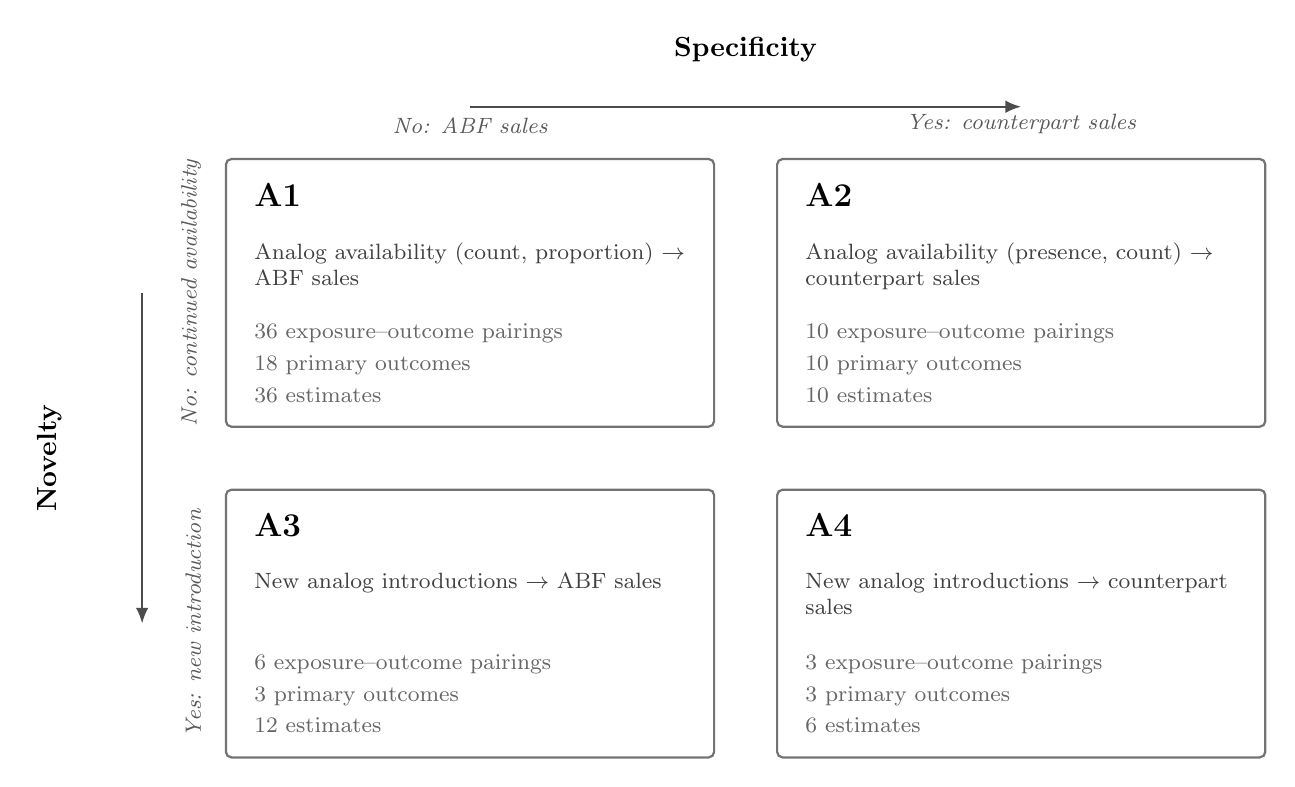
\begin{tikzpicture}[
  font=\small,
  axis label/.style  = {font=\bfseries},
  level/.style       = {font=\itshape\footnotesize, text=black!65},
  cell/.style        = {draw=black!55, thick, rounded corners=2pt,
                        minimum width=62mm, minimum height=34mm,
                        align=left, inner sep=8pt, anchor=north west},
  alabel/.style      = {font=\bfseries\large},
  desc/.style        = {font=\footnotesize, text=black!75},
  countline/.style   = {font=\footnotesize, text=black!60},
  arr/.style         = {-{Latex[length=2.0mm,width=1.6mm]},
                        thick, color=black!70},
]

% =============================================================
% Grid cells (2 x 2)
% =============================================================
% Cell positions are anchored at their north-west corner.
% Column x-coords:  left col @ 0,   right col @ 7.0
% Row    y-coords:  top row @ 0,    bottom row @ -3.8
\node[cell] (A1) at (0.0,  0.0) {};
\node[cell] (A2) at (7.0,  0.0) {};
\node[cell] (A3) at (0.0, -4.2) {};
\node[cell] (A4) at (7.0, -4.2) {};

% --- A1: no novelty, no specificity ---
\node[alabel, anchor=north west] at ($(A1.north west)+(0.25,-0.20)$) {A1};
\node[desc,   anchor=north west, text width=55mm]
  at ($(A1.north west)+(0.25,-0.95)$)
  {Analog availability (count, proportion) $\rightarrow$ ABF sales};
\node[countline, anchor=south west] at ($(A1.south west)+(0.25,0.95)$)
  {36 exposure--outcome pairings};
\node[countline, anchor=south west] at ($(A1.south west)+(0.25,0.55)$)
  {18 primary outcomes};
\node[countline, anchor=south west] at ($(A1.south west)+(0.25,0.20)$)
  {36 estimates};

% --- A2: no novelty, yes specificity ---
\node[alabel, anchor=north west] at ($(A2.north west)+(0.25,-0.20)$) {A2};
\node[desc,   anchor=north west, text width=55mm]
  at ($(A2.north west)+(0.25,-0.95)$)
  {Analog availability (presence, count) $\rightarrow$ counterpart sales};
\node[countline, anchor=south west] at ($(A2.south west)+(0.25,0.95)$)
  {10 exposure--outcome pairings};
\node[countline, anchor=south west] at ($(A2.south west)+(0.25,0.55)$)
  {10 primary outcomes};
\node[countline, anchor=south west] at ($(A2.south west)+(0.25,0.20)$)
  {10 estimates};

% --- A3: yes novelty, no specificity ---
\node[alabel, anchor=north west] at ($(A3.north west)+(0.25,-0.20)$) {A3};
\node[desc,   anchor=north west, text width=55mm]
  at ($(A3.north west)+(0.25,-0.95)$)
  {New analog introductions $\rightarrow$ ABF sales};
\node[countline, anchor=south west] at ($(A3.south west)+(0.25,0.95)$)
  {6 exposure--outcome pairings};
\node[countline, anchor=south west] at ($(A3.south west)+(0.25,0.55)$)
  {3 primary outcomes};
\node[countline, anchor=south west] at ($(A3.south west)+(0.25,0.20)$)
  {12 estimates};

% --- A4: yes novelty, yes specificity ---
\node[alabel, anchor=north west] at ($(A4.north west)+(0.25,-0.20)$) {A4};
\node[desc,   anchor=north west, text width=55mm]
  at ($(A4.north west)+(0.25,-0.95)$)
  {New analog introductions $\rightarrow$ counterpart sales};
\node[countline, anchor=south west] at ($(A4.south west)+(0.25,0.95)$)
  {3 exposure--outcome pairings};
\node[countline, anchor=south west] at ($(A4.south west)+(0.25,0.55)$)
  {3 primary outcomes};
\node[countline, anchor=south west] at ($(A4.south west)+(0.25,0.20)$)
  {6 estimates};

% =============================================================
% Column headers (Specificity axis)
% =============================================================
\node[axis label, anchor=south]
  at ($(A1.north)!0.5!(A2.north) + (0,1.10)$) {Specificity};

\node[level, anchor=south]
  at ($(A1.north) + (0,0.18)$) {No: ABF sales};
\node[level, anchor=south]
  at ($(A2.north) + (0,0.18)$) {Yes: counterpart sales};

% horizontal arrow under "Specificity" header showing direction
\draw[arr]
  ($(A1.north) + (0,0.65)$) -- ($(A2.north) + (0,0.65)$);

% =============================================================
% Row headers (Novelty axis)
% =============================================================
\node[axis label, rotate=90, anchor=south]
  at ($(A1.west)!0.5!(A3.west) + (-1.95,0)$) {Novelty};

\node[level, rotate=90, anchor=south]
  at ($(A1.west) + (-0.18,0)$) {No: continued availability};
\node[level, rotate=90, anchor=south]
  at ($(A3.west) + (-0.18,0)$) {Yes: new introduction};

% vertical arrow next to "Novelty" header showing direction
\draw[arr]
  ($(A1.west) + (-1.05,0)$) -- ($(A3.west) + (-1.05,0)$);

\end{tikzpicture}
\end{document}
